\section{\rev{Information Retention and Alternative Subgraph Selection}}
\label{sec:s13-retention}
\begin{revisionblock}
\subsection{Evaluation design and selection policies}
We assess compression through graph structure, frozen-encoder representations, and generated answers, fixing candidate identities and fuzzy input order (raw/display-control for repoDB). All variants reuse 2,100 validation and 2,100 test rows; unchanged candidate ranking is therefore a design constraint, not evidence of information retention.

\paragraph{Source graphs and matched budgets.}
Uncompressed references retain either all retrieved edge occurrences or unique directed, relation-labeled triples. Compressed alternatives select from the same unique source triples and match the original fuzzy graph's unique-edge count per query. An empty-local-graph reference retains frozen global embeddings. These three references have different budgets from the compressed selectors.

\paragraph{Selection strategies.}
We compare uniform random sampling without replacement, random coverage-first selection, native-score top-$B$, strict native-score coverage-then-fill, endpoint-degree top-$B$, breadth-first ordering, query- and terminal-personalized PageRank, shortest paths, and relation-stratified selection. Native scores use the original features with aligned triples and candidates; the strict coverage control omits dataset-specific reservation passes.

PageRank uses an unweighted undirected graph, damping 0.85, and uniform teleportation to the query or to the query and present candidates; dangling mass returns to this distribution. Iteration stops at L1 change below $10^{-10}$ or 200 steps, and endpoint-score sums rank edges. Shortest-path selection visits candidates in fixed order, adds a complete path of at most three edges when it fits, and fills remaining slots by native score. Relation-stratified selection cycles through relation IDs using within-relation native scores. Nonrandom ties follow source order, and no selector uses held-out gold labels.

Matched-budget random selection uses five seeds. Strict-budget curves use 20\%, 35\%, 55\%, 75\%, and 90\% of unique source edges, with three random seeds. We also vary the original policy's requested budget while retaining its reservation rules, reporting any excess separately from strict-budget results.

\paragraph{Retention metrics.}
Candidate coverage is incidence to at least one retained edge, measured absolutely and relative to source-covered candidates. For source graph $G_q$ and selected graph $S_q$, let $C_{\leq k}$ denote candidates reachable within $k$ edges and $P_k$ the edge-labeled simple paths of length $k$ ending at a candidate. For $k\in\{2,3\}$,
\[
 R_{\mathrm{reach},k}(q)=
 \frac{|C_{\leq k}(S_q)|}{|C_{\leq k}(G_q)|},\qquad
 R_{\mathrm{path},k}(q)=
 \frac{|\{p\in P_k(G_q):E(p)\subseteq E(S_q)\}|}{|P_k(G_q)|}.
\]
Paths allow traversal in either direction while retaining edge identities, relation labels, and traversal signs; they measure structural connectivity rather than biochemical mechanisms. Typed-pattern retention requires at least one surviving witness for each source relation/sign sequence. Incoming-context retention measures unique edges within two predecessor steps of the query and candidates, corresponding to the encoder's two directed message-passing layers.

Additional metrics cover query presence, nodes, relation types, direct query--candidate edges, and base-2 Jensen--Shannon divergence of relation and node-incidence distributions. Rare-relation recall uses source frequencies at or below the per-query median. Means average per-row ratios, excluding zero-denominator rows and reporting eligible counts.

\paragraph{Frozen-model evaluation and uncertainty.}
We evaluate 22 primary variants and six strict-budget variants (native-score coverage, terminal PageRank, and random seed zero at 35\% and 75\%) on the complete test split. Within each dataset, checkpoint, prompt, candidate order, and deterministic decoding are fixed. Query/candidate adapter outputs are compared with both source references using cosine similarity and relative L2 change; answer evaluation follows Section~\ref{sec:s12-calibration}. Graphs with at most ten edge occurrences use global embeddings without local message passing.

Exploratory 95\% intervals use 2,000 paired query-cluster bootstrap resamples, with joint query/seed resampling for random-selector means and no multiplicity adjustment. Seed standard deviations are reported separately. Configurations are fixed before inference, and test outcomes do not select a new default.

\subsection{Structural retention results and compression trade-offs}
\paragraph{Duplicate and unique-edge removal.}
PrimeKG averages 59.932 source edge occurrences, 38.094 unique triples, and 32.340 retained fuzzy triples per test row. Of the 27.592-occurrence reduction, 21.838 (79.1\%) are duplicates and 5.754 are unique triples. The other four datasets contain no source duplicates in these inputs. Duplicate removal can still affect repeated encoder messages. Table~\ref{tab:s25-all-reachability} compares reachability across all selectors.

\par\addvspace{0.8\baselineskip}\noindent\begin{minipage}{\linewidth}

\centering\small\setlength{\tabcolsep}{4pt}
\captionof{table}{Full matched-budget comparison of three-hop reachability retention. Random rows average all five seeds. Eligible row counts are 488, 500, 90, 386, and 297 for PrimeKG, PharmKG, Hetionet, DRKG, and repoDB. Candidate order and unique-edge count are fixed per query.}
\label{tab:s25-all-reachability}
\begin{tabular}{lrrrrr}
\toprule
Selector & PrimeKG & PharmKG & Hetionet & DRKG & repoDB \\
\midrule
Original fuzzy & 0.7737 & 0.9010 & 0.4835 & 0.8921 & 0.9546 \\
Native score top-$k$ & 0.7805 & 0.5600 & 0.1455 & 0.0922 & 0.0000 \\
Strict native coverage & 0.7737 & 0.9069 & 0.4835 & 0.6242 & 0.5634 \\
Degree top-$k$ & 0.8408 & 0.5532 & 0.6251 & 0.5734 & 0.2591 \\
Query BFS & 0.8328 & 0.6254 & 0.7047 & 0.8075 & 0.9164 \\
Query PPR & 0.7868 & 0.6021 & 0.6814 & 0.7940 & 0.9005 \\
Terminal PPR & 0.9111 & 0.5972 & 0.6251 & 0.7305 & 0.9112 \\
Shortest paths & 0.9985 & 1.0000 & 1.0000 & 1.0000 & 1.0000 \\
Relation stratified & 0.7694 & 0.8429 & 0.8479 & 0.6974 & 0.9399 \\
Random (5 seeds) & 0.7760 & 0.4423 & 0.4848 & 0.5043 & 0.5465 \\
Random + coverage (5 seeds) & 0.7816 & 0.7465 & 0.6068 & 0.7125 & 0.7700 \\
\bottomrule
\end{tabular}


\end{minipage}\par\medskip

\paragraph{Coverage and path preservation.}
Fuzzy retrieval retains incident evidence for all source-covered candidates, but its reachability exceeds random selection only on PharmKG, DRKG, and repoDB. The exploratory random-minus-fuzzy intervals are $[-0.4829,-0.4337]$, $[-0.4433,-0.3353]$, and $[-0.4492,-0.3661]$, respectively; PrimeKG and Hetionet intervals include zero. Shortest-path selection preserves nearly all source connectivity but reduces candidate coverage to 0.8514 on Hetionet, 0.8199 on DRKG, and 0.8971 on repoDB. Thus, candidate incidence and query-connected paths favor different selection policies.

\par\addvspace{0.8\baselineskip}\noindent\begin{minipage}{\linewidth}

\centering\small
\captionof{table}{Exact edge-labeled path retention at length three. $N$ counts rows with at least one source path; zero-denominator rows are excluded. Random is mean $\pm$ seed standard deviation. Paths are structural witnesses, not validated therapeutic mechanisms.}
\label{tab:s26-paths}
\begin{tabular}{lrrrr}
\toprule
Dataset & $N$ & Fuzzy & Random (5 seeds) & Shortest paths \\
\midrule
PrimeKG & 488 & 0.6543 & $0.6443\pm0.0047$ & 0.8199 \\
PharmKG & 31 & 0.0000 & $0.1801\pm0.0967$ & 0.8604 \\
Hetionet & 64 & 0.0000 & $0.1615\pm0.0589$ & 0.6207 \\
DRKG & 201 & 0.4767 & $0.1629\pm0.0078$ & 0.6496 \\
repoDB & 219 & 0.5286 & $0.1552\pm0.0185$ & 0.8322 \\
\bottomrule
\end{tabular}


\end{minipage}\par\medskip

Table~\ref{tab:s26-paths} shows losses hidden by candidate coverage: fuzzy retrieval retains no length-three paths in eligible PharmKG or Hetionet rows, although shorter paths can survive and only 31 PharmKG rows contain such source paths. It retains more length-three paths than random on DRKG and repoDB. Table~\ref{tab:s27-other-retention} provides complementary structural diagnostics.

\par\addvspace{0.8\baselineskip}\noindent\begin{minipage}{\linewidth}

\centering\small\setlength{\tabcolsep}{4pt}
\captionof{table}{Complementary retention diagnostics for original fuzzy retrieval. Nodes and relation types are retained fractions; relation JSD is base-2 Jensen--Shannon divergence (zero means identical distributions). Incoming-2 measures directed incoming context within two predecessor steps. Rare edges belong to relations with frequency at or below the source median.}
\label{tab:s27-other-retention}
\begin{tabular}{lrrrrr}
\toprule
Dataset & Nodes & Relation types & Relation JSD & Incoming-2 & Rare edges \\
\midrule
PrimeKG & 0.9402 & 0.9378 & 0.0046 & 0.8593 & 0.8069 \\
PharmKG & 0.5735 & 0.8984 & 0.1375 & 0.6180 & 0.8774 \\
Hetionet & 0.5868 & 0.8370 & 0.0438 & 0.4309 & 0.5330 \\
DRKG & 0.5701 & 0.6562 & 0.0708 & 0.6100 & 0.4644 \\
repoDB & 0.5102 & 0.8582 & 0.0319 & 0.5433 & 0.6319 \\
\bottomrule
\end{tabular}


\end{minipage}\par\medskip

\paragraph{Budget feasibility.}
The original PrimeKG coverage-first policy can exceed smaller requested budgets: at 20\% of unique source edges, mean requested/actual counts are 7.576/15.662, with excess in 99.8\% of test rows; at 35\%, they are 13.336/15.886 and 74.2\%. No excess occurs at the original budgets used for the matched comparison. Strict-budget curves therefore report a separate policy with enforced limits.

\subsection{Frozen-model representation and generated-answer results}
Tables~\ref{tab:s28-selector-accuracy} and~\ref{tab:s29-encoder} summarize accuracy, encoder changes, and answer agreement under fixed candidate order. The 28 variants per dataset use the same frozen checkpoint and matching rules from Section~\ref{sec:s12-calibration}.

\par\addvspace{0.8\baselineskip}\noindent\begin{minipage}{\linewidth}

\centering\small
\captionof{table}{Exact generated-answer accuracy (\%) under the standardized matching
rule. Random rows average all five seeds. Source raw/unique and empty local
graph are diagnostic references with different budgets; the other rows use
matched unique-edge budgets. The source multiset uses the original fuzzy input candidate order, so it is an order-matched graph reference rather than the raw-candidate baseline.}
\label{tab:s28-selector-accuracy}
\begin{tabular}{lrrrrr}
\toprule
Selector & PrimeKG & PharmKG & Hetionet & DRKG & repoDB \\
\midrule
Source multiset & 0.00 & 0.00 & 3.00 & 1.40 & 0.20 \\
Source unique & 0.00 & 0.00 & 3.00 & 1.40 & 0.20 \\
Empty local graph & 0.40 & 0.00 & 1.00 & 1.20 & 1.80 \\
Original fuzzy & 0.00 & 0.20 & 3.00 & 1.40 & 0.40 \\
Native score top-$k$ & 0.00 & 0.00 & 2.00 & 1.20 & 2.20 \\
Strict native coverage & 0.00 & 0.20 & 3.00 & 1.40 & 0.40 \\
Degree top-$k$ & 0.00 & 0.20 & 0.00 & 1.20 & 1.60 \\
Query BFS & 0.00 & 0.20 & 0.00 & 1.20 & 0.40 \\
Query PPR & 0.00 & 0.20 & 0.00 & 1.20 & 0.40 \\
Terminal PPR & 0.00 & 0.20 & 2.00 & 1.20 & 0.40 \\
Shortest paths & 0.00 & 0.20 & 3.00 & 1.40 & 0.20 \\
Relation stratified & 0.00 & 0.00 & 2.00 & 1.20 & 0.20 \\
Random (5 seeds) & 0.04 & 0.04 & 3.00 & 1.24 & 0.52 \\
Random + coverage (5 seeds) & 0.00 & 0.08 & 3.00 & 1.40 & 0.16 \\
\bottomrule
\end{tabular}


\end{minipage}\par\medskip



\par\addvspace{0.8\baselineskip}\noindent\begin{minipage}{\linewidth}

\centering\small
\captionof{table}{Original fuzzy versus the uncompressed source: encoder output changes
and normalized generated-answer agreement. Candidate metrics average the 20
candidate embeddings within each row, then average rows. A cosine near one
does not exclude a change in vector magnitude; relative L2 is reported
separately.}
\label{tab:s29-encoder}
\resizebox{\linewidth}{!}{\begin{tabular}{lrrrrr}
\toprule
Dataset & Query cosine & Candidate cosine & Query rel. L2 & Candidate rel. L2 & Agreement (\%) \\
\midrule
PrimeKG & 0.8828 & 0.9453 & 0.8818 & 0.1013 & 78.8 \\
PharmKG & 0.8718 & 0.9991 & 0.6130 & 0.0032 & 80.0 \\
Hetionet & 0.9209 & 1.0000 & 0.3259 & 0.0000 & 100.0 \\
DRKG & 0.9312 & 0.9867 & 0.3834 & 0.0526 & 100.0 \\
repoDB & 0.9814 & 0.9806 & 0.1326 & 0.0862 & 80.8 \\
\bottomrule
\end{tabular}
}

\end{minipage}\par\medskip

\paragraph{Structural loss and output agreement.}
On Hetionet, fuzzy retrieval preserves candidate encoder outputs (cosine 1.0000; relative L2 0.0000) and generated answers, despite changed query outputs (cosine 0.9209; relative L2 0.3259) and complete loss of eligible length-three paths. DRKG also retains all answers despite representation changes. Output agreement therefore does not establish whole-graph preservation. Answer agreement falls to 78.8\%, 80.0\%, and 80.8\% on PrimeKG, PharmKG, and repoDB, respectively.

No selector consistently dominates downstream accuracy. On repoDB, fuzzy retrieval produces 2/500 correct answers, compared with 1/500 for the uncompressed source, 11/500 for native-score top-$k$, and 9/500 for the empty-local-graph reference, which still uses global embeddings. Fuzzy retrieval yields 0/500, 1/500, 3/100, and 7/500 on PrimeKG, PharmKG, Hetionet, and DRKG. These low counts limit claims about small gains; a bootstrap interval including zero does not establish equivalence. Full paired comparisons are provided in the result workbook.

\subsection{Budget--retention curves}
Figures~\ref{fig:c3-duplicates}--\ref{fig:c3-budget-paths} show duplicate removal and retention across strict budgets expressed as fractions of unique source triples. The strict coverage control is distinguished from the original dataset-specific policy.

\par\addvspace{0.8\baselineskip}\noindent\begin{minipage}{\linewidth}

\centering
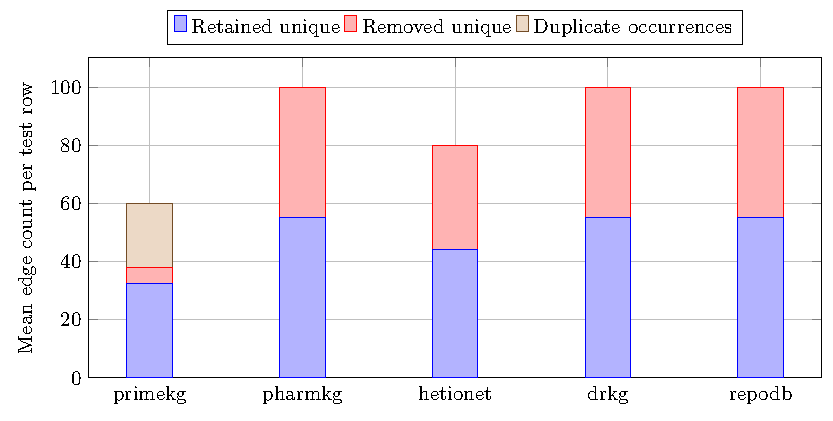
\includegraphics[width=.96\textwidth]{revision_figures/compression_decomposition.pdf}
\captionof{figure}{Decomposition of source edge occurrences into retained unique triples,
removed unique triples, and duplicate occurrences. Counts are means over test
rows; duplicate removal is separated from structural edge loss.}
\label{fig:c3-duplicates}

\end{minipage}\par\medskip



\par\addvspace{0.8\baselineskip}\noindent\begin{minipage}{\linewidth}

\centering
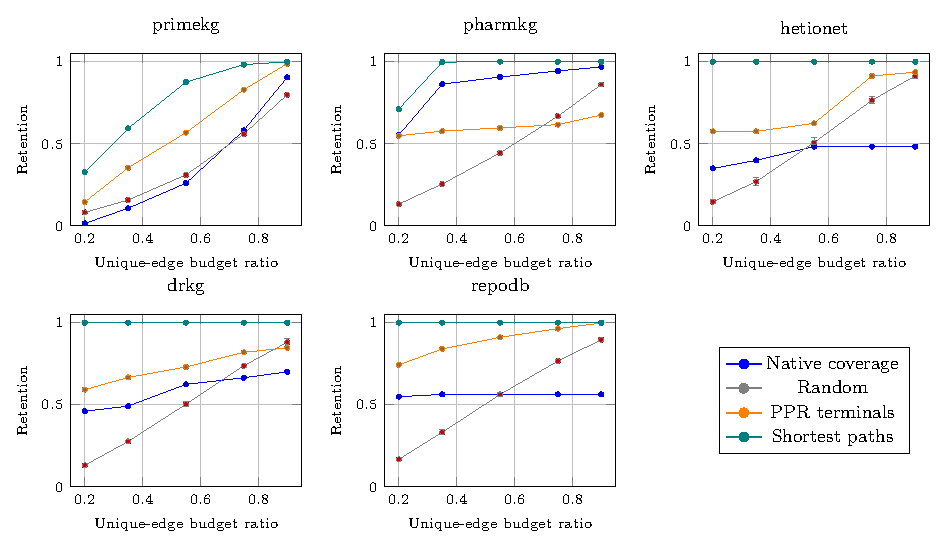
\includegraphics[width=.98\textwidth]{revision_figures/budget_reach3_retention.pdf}
\captionof{figure}{Candidate--query reachability retention for strict-budget selectors.
The native-score coverage control is distinguished from the original
dataset-specific selector. Random error bars show seed variability, not test
confidence intervals. Native implementation budget violations are reported
separately in the audit tables.}
\label{fig:c3-budget-reach}

\end{minipage}\par\medskip



\par\addvspace{0.8\baselineskip}\noindent\begin{minipage}{\linewidth}

\centering
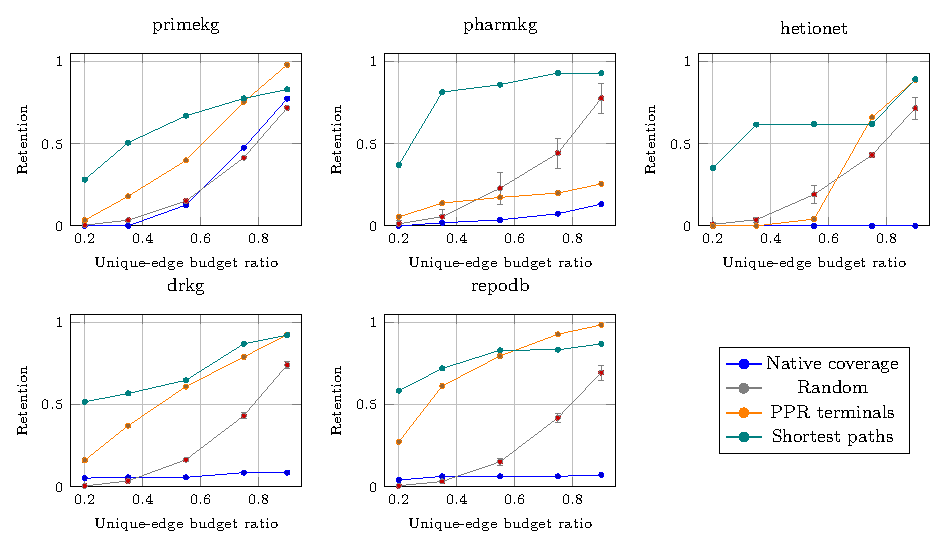
\includegraphics[width=.98\textwidth]{revision_figures/budget_path3_retention.pdf}
\captionof{figure}{Exact length-three path-witness retention under the same strict-budget
controls. Means exclude queries without a corresponding source witness;
eligible counts are provided in the accompanying tables.}
\label{fig:c3-budget-paths}

\end{minipage}\par\medskip

\end{revisionblock}
